\section{Experiment 4}\label{sec:experiment-4}

In this experiment, a machine learning pipeline is used to explore how the performance of linear and nonlinear dimensionality reduction methods compare using different sizes of samples.

Overall, the results of this experiment provide insight into the factors that can influence the effectiveness of dimensionality reduction in machine learning and can inform the choice of dimensionality reduction method in real-world scenarios. Furthermore, the findings can contribute to the broader understanding of the role of sample size in choices of dimensionality reduction and its effect on machine learning models, which is relevant especially when working with cross validation.

\subsection{Rules and overview of the experiment}
This experiment uses the original hyperparameters. These can also be read in \autoref{subsubsec:the-hyperparameters}. The difference is that it will be used on datasamples from \gls{mnist} of the size 200, 300, 400, 500, 600, 700, 800, 900, 1000, 2000, 3000, 4000, 5000.

This experiment is run on pc-4. See \autoref{tab:pc4-specs} for the specific specs for the computer used in the experiment.


\subsection{Results}\label{subsec:experiment_4_results}
This section presents the results of the fourth experiment, which compares the performance of different dimensionality reduction methods on a classification task. The results are shown for different sample sizes using confusion matrices, tables of the classification reports, and scatter plots, which visualize the relationship between sample size, accuracy, and time taken.

The results are evaluated based on the rules of the experiment, focusing on accuracy, F1 score, and time taken. The specific accuracy values obtained from the experiment's CSV files are also discussed. The scatter plots provide a visual representation of the results and enable the comparison of when the different methods accuracy and time start to rise. In general, the results for each method and the base case will show the results for samples of sizes of 200, 1000 and 5000 in detail.

\subsubsection{Support vector machine model}\label{subsubsec:experiment_4_no_dimmensionality_reduction}


\begin{table}[htb!]
\centering
\begin{tabular}{lrrrr}
    \toprule
 & precision & recall & f1-score & support \\
 \midrule
 0 & 83.0224 & 90.8163 & 86.7446 & 980 \\
 1 & 78.2424 & 97.2687 & 86.7243 & 1135 \\
 2 & 67.8335 & 69.4767 & 68.6453 & 1032 \\
 3 & 73.6059 & 78.4158 & 75.9348 & 1010 \\
 4 & 70.7377 & 87.8819 & 78.3833 & 982 \\
 5 & 71.6243 & 41.0314 & 52.1739 & 892 \\
 6 & 91.3043 & 63.5699 & 74.9538 & 958 \\
 7 & 78.3178 & 81.5175 & 79.8856 & 1028 \\
 8 & 73.1092 & 71.4579 & 72.2741 & 974 \\
 9 & 71.7842 & 68.5828 & 70.1470 & 1009 \\
 accuracy & & & 756700 & 10000 \\
 macro avg & 75.9582 & 75.0019 & 74.5867 & 10000 \\
 weighted avg & 75.9485 & 75.6700 & 74.9591 & 10000 \\
 \bottomrule
\end{tabular}
\caption{Classification report for baseline\_svm\_200}
\label{tab:classification-report-baseline_svm_200}
\end{table}

\begin{table}[htb!]
\centering
\caption{Classification report for baseline_svm_1000}
\label{tab:classification-report-baseline_svm_1000}
\begin{tabular}{lrrrr}
\toprule
 & precision & recall & f1-score & support \\
\midrule
0 & 0.925998 & 0.970408 & 0.947683 & 980.000000 \\
1 & 0.921667 & 0.974449 & 0.947323 & 1135.000000 \\
2 & 0.865842 & 0.881783 & 0.873740 & 1032.000000 \\
3 & 0.877095 & 0.777228 & 0.824147 & 1010.000000 \\
4 & 0.867005 & 0.869654 & 0.868327 & 982.000000 \\
5 & 0.785340 & 0.840807 & 0.812128 & 892.000000 \\
6 & 0.914621 & 0.894572 & 0.904485 & 958.000000 \\
7 & 0.860927 & 0.885214 & 0.872902 & 1028.000000 \\
8 & 0.864350 & 0.791581 & 0.826367 & 974.000000 \\
9 & 0.822178 & 0.815659 & 0.818905 & 1009.000000 \\
accuracy & 0.871700 & 0.871700 & 0.871700 & 0.871700 \\
macro avg & 0.870502 & 0.870136 & 0.869601 & 10000.000000 \\
weighted avg & 0.871760 & 0.871700 & 0.871014 & 10000.000000 \\
\bottomrule
\end{tabular}
\end{table}

\begin{table}[htb!]
\centering
\begin{tabular}{lrrrr}
    \toprule
    & precision & recall & f1-score & support \\
    \midrule
    0 & 0.955224 & 0.979592 & 0.967254 & 980.000000 \\
    1 & 0.953072 & 0.984141 & 0.968357 & 1135.000000 \\
    2 & 0.909980 & 0.901163 & 0.905550 & 1032.000000 \\
    3 & 0.890279 & 0.915842 & 0.902879 & 1010.000000 \\
    4 & 0.904854 & 0.949084 & 0.926441 & 982.000000 \\
5 & 0.901278 & 0.869955 & 0.885339 & 892.000000 \\
6 & 0.952128 & 0.934238 & 0.943098 & 958.000000 \\
7 & 0.925123 & 0.913424 & 0.919236 & 1028.000000 \\
8 & 0.904555 & 0.856263 & 0.879747 & 974.000000 \\
9 & 0.902414 & 0.888999 & 0.895657 & 1009.000000 \\
accuracy & 0.920500 & 0.920500 & 0.920500 & 0.920500 \\
macro avg & 0.919891 & 0.919270 & 0.919356 & 10000.000000 \\
weighted avg & 0.920338 & 0.920500 & 0.920197 & 10000.000000 \\
\bottomrule
\end{tabular}
\caption{Classification report for baseline\_svm\_5000}
\label{tab:classification-report-baseline_svm_5000}
\end{table}


The results of this experiment are shown in \autoref{tab:classification-report-baseline_svm_200}. The table shows the precision, recall, and f1-score for each of the ten classes in the dataset and the overall accuracy of the model. The table also shows the macro average and weighted average scores.

Overall, the results show that the \gls{svm} model achieved an accuracy of approximately 67\%. This indicates that the model performed relatively well but still had some errors in its predictions. The precision and recall scores for each class varied, with some classes having higher scores than others. For example, the model had a precision of approximately 87\% for class 0 but only a precision of approximately 45\% for class 9.

These results provide a baseline for comparison with the results of the other parts of the experiment, in which different dimensionality reduction methods were applied. The results of this initial experiment will be used to evaluate the effectiveness of the different dimensionality reduction methods in improving the performance of the \gls{svm} model.

The second part of the base case involved using a sample size of 1000; it can be seen in \ref{tab:classification-report-baseline_svm_1000}. Compared to the results of the first part of the experiment, the accuracy of the \gls{svm} model improved significantly, achieving an accuracy of approximately 87\%. This indicates that using a larger sample size improved the performance of the model. The precision and recall scores for each class also improved, with most classes having higher scores than in the first part of the experiment.

The following sample of size 5000 can be seen in \autoref{tab:classification-report-baseline_svm_5000}. Comparing \autoref{tab:classification-report-baseline_svm_5000} and \autoref{tab:classification-report-baseline_svm_5000}, it is clear that the \gls{svm} model achieved higher accuracy and precision when trained on a larger sample size. For example, the accuracy of the model increased from 87\% for the 1000-sample dataset to 92\% for the 5000-sample dataset. Similarly, the precision of the model increased for most of the classes, with the most significant increase being seen for class 5, where the precision increased from 78\% to 90\%.

Additionally, the f1-score, which is a measure of the balance between precision and recall, also improved for most classes when using a larger sample size. This suggests that the model was able to make more accurate predictions and avoid false positives and false negatives more effectively when trained on a larger dataset.


\subsubsection{Principal component analysis}\label{subsubsec:experiment_4_pca}

The second part of the experiment involved running a machine learning pipeline applying \gls{pca} as a dimensionality reduction method. The sample sizes for this part of the experiment were 200, 1000, and 5000.

\begin{table}[htb!]
\centering
\caption{Classification report for pca_svm_200}
\label{tab:classification-report-pca_svm_200}
\begin{tabular}{lrrrr}
\toprule
 & precision & recall & f1-score & support \\
\midrule
0 & 0.838207 & 0.877551 & 0.857428 & 980.000000 \\
1 & 0.770701 & 0.959471 & 0.854788 & 1135.000000 \\
2 & 0.675052 & 0.624031 & 0.648540 & 1032.000000 \\
3 & 0.744227 & 0.829703 & 0.784644 & 1010.000000 \\
4 & 0.692244 & 0.845214 & 0.761119 & 982.000000 \\
5 & 0.747492 & 0.501121 & 0.600000 & 892.000000 \\
6 & 0.931649 & 0.654489 & 0.768853 & 958.000000 \\
7 & 0.832487 & 0.797665 & 0.814704 & 1028.000000 \\
8 & 0.737317 & 0.671458 & 0.702848 & 974.000000 \\
9 & 0.641791 & 0.724480 & 0.680633 & 1009.000000 \\
accuracy & 0.754000 & 0.754000 & 0.754000 & 0.754000 \\
macro avg & 0.761117 & 0.748518 & 0.747356 & 10000.000000 \\
weighted avg & 0.760509 & 0.754000 & 0.750028 & 10000.000000 \\
\bottomrule
\end{tabular}
\end{table}


This classification report shows the performance of a \gls{svm} model that has been trained using \gls{pca}. The result of the first sample of 200 can be seen in \ref{tab:classification-report-pca_svm_200}
For example, class 0 has a precision of 84\% and a recall of 88\%, while class 9 has a precision of 64\% and a recall of 72\%. This indicates that the model is more accurate at correctly identifying instances of class 0 than it is at correctly identifying instances of class 9. The f1-score for class 0 is 86\%, while the f1-score for class 9 is 68\%, further highlighting the difference in performance between the two classes. Overall, it appears that class 0 and class 9 have the largest differences in performance on this classification report.

\begin{table}[htb!]
\centering
\caption{Classification report for pca_svm_1000}
\label{tab:classification-report-pca_svm_1000}
\begin{tabular}{lrrrr}
\toprule
 & precision & recall & f1-score & support \\
\midrule
0 & 0.928358 & 0.952041 & 0.940050 & 980.000000 \\
1 & 0.956484 & 0.968282 & 0.962347 & 1135.000000 \\
2 & 0.885417 & 0.906008 & 0.895594 & 1032.000000 \\
3 & 0.898343 & 0.804950 & 0.849086 & 1010.000000 \\
4 & 0.910510 & 0.891039 & 0.900669 & 982.000000 \\
5 & 0.818376 & 0.858744 & 0.838074 & 892.000000 \\
6 & 0.921244 & 0.927975 & 0.924597 & 958.000000 \\
7 & 0.899497 & 0.870623 & 0.884825 & 1028.000000 \\
8 & 0.840256 & 0.810062 & 0.824882 & 974.000000 \\
9 & 0.808081 & 0.872151 & 0.838894 & 1009.000000 \\
accuracy & 0.887400 & 0.887400 & 0.887400 & 0.887400 \\
macro avg & 0.886656 & 0.886187 & 0.885902 & 10000.000000 \\
weighted avg & 0.888159 & 0.887400 & 0.887261 & 10000.000000 \\
\bottomrule
\end{tabular}
\end{table}


In \ref{tab:classification-report-pca_svm_1000} it can see that overall, the second model (pca\_svm\_1000) performs better on the classification task than the first model (pca\_svm\_200), as shown by the higher accuracy, precision, recall, and f1-score values for most classes in the second report. For example, class 0 has a precision of 91\% and a recall of 96\% in the second report, compared to 83\% and 88\% in the first report. The f1-score for class 0 is also higher in the second report (94\%) than in the first report (85\%).

One interesting difference between the two reports is the performance on class 3. In the first report, class 3 has a recall of 83\%, with an f1-score of 78\%. In the second report, class 3 had a lower recall of 79\%, resulting in a f1-score of 83\%. This indicates that the second model (pca\_svm\_1000) is less accurate at correctly identifying instances of class 3 than the first model the f1 score is still higher due to the precision being suitably higher to compensate(pca\_svm\_200).

The last model is seen in \autoref{tab:classification-report-pca_svm_5000} and is overall, the pca\_svm\_5000 model appears to have better performance across most of the metrics, with higher values for precision, recall, and f1-score for most of the classes.

\begin{table}[htb!]
    \centering
    \begin{tabular}{lrrrr}
        \toprule
                     & precision & recall  & f1-score & support \\
        \midrule
        0            & 94.0476   & 96.7347 & 95.3722  & 980     \\
        1            & 95.8656   & 98.0617 & 96.9512  & 1135    \\
        2            & 89.0927   & 89.4380 & 89.2650  & 1032    \\
        3            & 86.6218   & 89.1089 & 87.8477  & 1010    \\
        4            & 90.7389   & 93.7882 & 92.2384  & 982     \\
        5            & 87.6417   & 86.6592 & 87.1477  & 892     \\
        6            & 93.6259   & 93.5282 & 93.5770  & 958     \\
        7            & 92.5000   & 89.9805 & 91.2229  & 1028    \\
        8            & 89.7577   & 83.6756 & 86.6100  & 974     \\
        9            & 89.1348   & 87.8097 & 88.4673  & 1009    \\
        accuracy     &           &         & 91.0000  & 10000   \\
        macro avg    & 90.9027   & 90.8785 & 90.8699  & 10000   \\
        weighted avg & 90.9832   & 91.0000 & 90.9711  & 10000   \\
        \bottomrule
    \end{tabular}
    \caption{Classification\ report\ for\ pca\_svm\_5000}
    \label{tab:classification-report-pca_svm_5000}
\end{table}



Overall, the results show that the \gls{svm} model using \gls{pca} achieved an accuracy of approximately 75\%, 77\%, and 84\% for the 200, 1000, and 5000 sample sizes, respectively. This indicates that the model performed relatively well, but still had some errors in its predictions. The precision and recall scores for each class varied, with some classes having higher scores than others. For example, the model had a precision of approximately 83\% for class 0 with a 200 sample size, but only a precision of approximately 64\% for class 9 with a 1000 sample size. Classes 0 and 9 showed the most significant differences in performance across the different sample sizes.

\subsubsection{Linear discriminant analysis}\label{subsubsec:experiment_4_lda}

\begin{table}[htb!]
\centering
\begin{tabular}{lrrrr}
    \toprule
 & precision & recall & f1-score & support \\
\midrule
0 & 80.1397 & 81.9388 & 81.0293 & 980 \\
1 & 60.4938 & 94.9780 & 73.9116 & 1135 \\
2 & 51.4586 & 42.7326 & 46.6914 & 1032 \\
3 & 66.7053 & 56.9307 & 61.4316 & 1010 \\
4 & 60.6034 & 69.5519 & 64.7700 & 982 \\
5 & 48.1481 & 20.4036 & 28.6614 & 892 \\
6 & 72.2449 & 55.4280 & 62.7289 & 958 \\
7 & 74.9458 & 67.2179 & 70.8718 & 1028 \\
8 & 59.0597 & 61.9097 & 60.4511 & 974 \\
9 & 43.7595 & 56.9871 & 49.5050 & 1009 \\
accuracy & & & 61.06200 & 10000 \\
macro avg & 61.7559 & 60.8078 & 60.0052 & 10000 \\
weighted avg & 61.8068 & 61.6200 & 60.4480 & 10000 \\
\bottomrule
\end{tabular}
\caption{Classification report for lda_svm_200}
\label{tab:classification-report-lda_svm_200}
\end{table}



This classification report seen in \autoref{tab:classification-report-lda_svm_200} shows the performance of a \gls{svm} model that has been trained using \gls{lda} on classifying handwritten digits from the \gls{mnist} dataset. For example, class 1 has a precision of 60\% and a recall of 94\%, while class 5 has a precision of 48\% and a recall of 20\%. This indicates that the model is more accurate at correctly identifying instances of class 1 than it is at correctly identifying instances of class 5. The f1-score for class 1 is 73\%, while the f1-score for class 5 is 28\%, further highlighting the difference in performance between the two classes. Overall, it appears that class 1 and class 5 have the largest differences in performance on this classification report.

\begin{table}[htb!]
\centering
\begin{tabular}{lrrrr}
    \toprule
    & precision & recall & f1-score & support \\
    \midrule
    0 & 69.9825 & 81.8367 & 75.4468 & 980 \\
    1 & 74.5657 & 94.5374 & 83.3722 & 1135 \\
    2 & 67.7530 & 38.2752 & 48.9164 & 1032 \\
    3 & 62.5000 & 51.9802 & 56.7568 & 1010 \\
    4 & 62.9767 & 68.9409 & 65.8240 & 982 \\
    5 & 49.6101 & 57.0628 & 53.0761 & 892 \\
    6 & 66.2461 & 65.7620 & 66.0031 & 958 \\
    7 & 64.8130 & 65.7588 & 65.2825 & 1028 \\
    8 & 59.4987 & 46.3039 & 52.0785 & 974 \\
    9 & 55.2239 & 62.3389 & 58.5661 & 1009 \\
    accuracy & & & 63.6700 & 10000 \\
    macro avg & 63.3170 & 63.2797 & 62.5323 & 10000 \\
    weighted avg & 63.6121 & 63.6700 & 62.8514 & 10000 \\
    \bottomrule
\end{tabular}
\caption{Classification report for lda_svm_1000}
\label{tab:classification-report-lda_svm_1000}
\end{table}


The classification report for lda\_svm\_1000 seen in \autoref{tab:classification-report-lda_svm_1000} shows generally better performance than the classification report for lda\_svm\_200. For example, class 1 has a precision of 74\% and a recall of 94\% in the lda\_svm\_1000 report, compared to a precision of 60\% and a recall of 94\% in the lda\_svm\_200 report. Additionally, the f1-score for class 1 is 83\% in the lda\_svm\_1000 report, compared to 73\% in the lda\_svm\_200 report. This indicates that the model trained on a larger sample size of 1000 has improved performance in correctly identifying instances of class 1. Overall, it appears that several classes, including 1, 3, 5, and 9, have seen improvements in precision, recall, and f1-score when trained on a larger sample size.


\begin{table}[htb!]
    \centering
    \begin{tabular}{lrrrr}
        \toprule
                     & precision & recall  & f1-score & support \\
        \midrule
        0            & 92.0039   & 95.1020 & 93.5273  & 980     \\
        1            & 90.7577   & 96.0352 & 93.3219  & 1135    \\
        2            & 87.1277   & 79.3605 & 83.0629  & 1032    \\
        3            & 85.4692   & 83.8614 & 84.6577  & 1010    \\
        4            & 82.7977   & 89.2057 & 85.8824  & 982     \\
        5            & 80.6306   & 80.2691 & 80.4494  & 892     \\
        6            & 88.1178   & 87.4739 & 87.7947  & 958     \\
        7            & 86.9347   & 84.1440 & 85.5166  & 1028    \\
        8            & 80.6999   & 78.1314 & 79.3949  & 974     \\
        9            & 80.7843   & 81.6650 & 81.2223  & 1009    \\
        accuracy     &           &         & 85.6800  & 10000   \\
        macro avg    & 85.5324   & 85.5248 & 85.4830  & 10000   \\
        weighted avg & 85.6542   & 85.6800 & 85.6202  & 10000   \\
        \bottomrule
    \end{tabular}
    \caption{Classification\ report\ for\ lda\_svm\_5000}
    \label{tab:classification-report-lda_svm_5000}
\end{table}


The classification report for lda\_svm\_5000 has higher precision, recall, and f1-score values for each class compared to the lda\_svm\_1000 report. For example, the precision for class 0 is 92\% in the lda\_svm\_5000 report, while it is 69\% in the lda\_svm\_1000 report. Similarly, the recall for class 0 is 95\% in the lda\_svm\_5000 report, while it is 81\% in the lda\_svm\_1000 report. The f1-score for class 0 is also higher in the lda\_svm\_5000 report (93\%) compared to the lda\_svm\_1000 report (75\%). Overall, it appears that the model trained on a larger sample size is more effective at correctly classifying instances in the \gls{mnist} dataset.

Based on these classification reports, the model with \gls{lda} is best at recognizing instances of class 1. This is because it has the highest precision and recall among all classes, as well as the highest f1-score. This indicates that the model is able to accurately identify instances of class 1 with a high degree of precision and recall. Furthermore, the difference in performance between class 1 and other classes is the largest, further highlighting the model's superior performance on this class. It also appears that the model is worst at recognizing classes 8, 9, 2 and 5.

\subsubsection{Kernel PCA}\label{subsubsec:experiment_4_kernel_pca}
In this part of the experiment it is expected that The performance of a \gls{svm} model using  \gls{kpca} for dimensionality reduction is likely to differ from that of an \gls{svm} model without \gls{kpca}. \gls{kpca} can reduce the dimensionality of a dataset by projecting it onto a lower-dimensional space, which can improve the \gls{svm} model's decision boundary and performance. In contrast, an \gls{svm} model without \gls{kpca} may be more sensitive to the curse of dimensionality and overfitting, especially on high-dimensional datasets.

\begin{table}[htb!]
    \centering
    \begin{tabular}{lrrrr}
        \toprule
                     & precision & recall  & f1-score & support \\
        \midrule
        0            & 75.2715   & 91.9388 & 82.7745  & 980     \\
        1            & 68.7965   & 97.7093 & 80.7426  & 1135    \\
        2            & 67.8387   & 63.5659 & 65.6328  & 1032    \\
        3            & 70.7317   & 74.6535 & 72.6397  & 1010    \\
        4            & 69.0129   & 81.8737 & 74.8952  & 982     \\
        5            & 76.9231   & 42.6009 & 54.8341  & 892     \\
        6            & 87.9245   & 72.9645 & 79.7490  & 958     \\
        7            & 87.5664   & 80.1556 & 83.6973  & 1028    \\
        8            & 79.3492   & 65.0924 & 71.5172  & 974     \\
        9            & 70.5394   & 67.3935 & 68.9306  & 1009    \\
        accuracy     &           &         & 74.4100  & 10000   \\
        macro avg    & 75.3954   & 73.7948 & 73.5413  & 10000   \\
        weighted avg & 75.2395   & 74.4100 & 73.7969  & 10000   \\
        \bottomrule
    \end{tabular}
    \caption{Classification\ report\ for\ kernel\_pca\_svm\_200}
    \label{tab:classification-report-kernel_pca_svm_200}
\end{table}



The values in \autoref{tab:classification-report-kernel_pca_svm_200} indicate that the model has relatively high precision and recall for most classes, with a few exceptions. Overall, the model has an accuracy of approximately 74\%.

\begin{table}[htb!]
    \centering
    \begin{tabular}{lrrrr}
        \toprule
                     & precision & recall  & f1-score & support \\
        \midrule
        0            & 91.2745   & 95.0000 & 93.1000  & 980     \\
        1            & 92.6236   & 97.3568 & 94.9313  & 1135    \\
        2            & 87.3466   & 89.6318 & 88.4744  & 1032    \\
        3            & 88.4279   & 80.1980 & 84.1121  & 1010    \\
        4            & 84.7573   & 88.9002 & 86.7793  & 982     \\
        5            & 79.0487   & 78.2511 & 78.6479  & 892     \\
        6            & 90.7466   & 90.0835 & 90.4138  & 958     \\
        7            & 88.4837   & 89.6887 & 89.0821  & 1028    \\
        8            & 85.0627   & 76.5914 & 80.6051  & 974     \\
        9            & 83.2847   & 84.9356 & 84.1021  & 1009    \\
        accuracy     &           &         & 87.3000  & 10000   \\
        macro avg    & 87.1056   & 87.0637 & 87.0248  & 10000   \\
        weighted avg & 87.2556   & 87.3000 & 87.2176  & 10000   \\
        \bottomrule
    \end{tabular}
    \caption{Classification\ report\ for\ kernel\_pca\_svm\_1000}
    \label{tab:classification-report-kernel_pca_svm_1000}
\end{table}


The classification report for kernel\_pca\_svm\_200 and kernel\_pca\_svm\_1000 show differences in the performance of the model on the two datasets. In general, the model trained on the larger dataset (kernel\_pca\_svm\_1000) which can be seen in \autoref{tab:classification-report-kernel_pca_svm_1000} appears to have higher precision, recall, and f1-scores for most classes.

\begin{table}[htb!]
\centering
\caption{Classification report for kernel_pca_svm_5000}
\label{tab:classification-report-kernel_pca_svm_5000}
\begin{tabular}{lrrrr}
\toprule
 & precision & recall & f1-score & support \\
\midrule
0 & 0.932485 & 0.972449 & 0.952048 & 980.000000 \\
1 & 0.950385 & 0.978855 & 0.964410 & 1135.000000 \\
2 & 0.915187 & 0.899225 & 0.907136 & 1032.000000 \\
3 & 0.898204 & 0.891089 & 0.894632 & 1010.000000 \\
4 & 0.901174 & 0.937882 & 0.919162 & 982.000000 \\
5 & 0.885417 & 0.857623 & 0.871298 & 892.000000 \\
6 & 0.924742 & 0.936326 & 0.930498 & 958.000000 \\
7 & 0.922772 & 0.906615 & 0.914622 & 1028.000000 \\
8 & 0.908207 & 0.863450 & 0.885263 & 974.000000 \\
9 & 0.892108 & 0.885035 & 0.888557 & 1009.000000 \\
accuracy & 0.914100 & 0.914100 & 0.914100 & 0.914100 \\
macro avg & 0.913068 & 0.912855 & 0.912763 & 10000.000000 \\
weighted avg & 0.913817 & 0.914100 & 0.913762 & 10000.000000 \\
\bottomrule
\end{tabular}
\end{table}


In general, the model trained on the larger dataset (kernel\_pca\_svm\_5000) which can be seen in \autoref{tab:classification-report-kernel_pca_svm_5000} appears to have higher precision, recall, and f1-scores for most classes. This suggests that, in this case, increasing the size of the dataset has led to a more accurate model.

Looking at the individual classes, some of the largest differences in performance can be seen in classes 1, 4, and 6. For class 1, the model trained on kernel\_pca\_svm\_5000 has a precision of 95\%, a recall of 97\%, and an f1-score of 96\%, while the model trained on kernel\_pca\_svm\_1000 has a precision of 92\%, a recall of 97\%, and an f1-score of 94\%. This indicates that the larger model is more effective at correctly identifying and classifying examples from class 1.

For class 4, the model trained on kernel\_pca\_svm\_5000 has a precision of 90\%, a recall of 93\%, and an f1-score of 91\%, while the model trained on kernel\_pca\_svm\_1000 has a precision of 84\%, a recall of 88\%, and an f1-score of 86\%. This indicates that the larger model is more effective at correctly identifying and classifying examples from class 4.

For class 6, the model trained on kernel\_pca\_svm\_5000 has a precision of 92\%, a recall of 93\%, and an f1-score of 93\%, while the model trained on kernel\_pca\_svm\_1000 has a precision of 90\%, a recall of 90\%, and an f1-score of 90\%. This indicates that the larger model is more effective at correctly identifying and classifying examples from class 6.

\subsubsection{ISOMAP embedding}\label{subsubsec:experiment_4_isomap}
This section presents the results of an experiment that was conducted to investigate the effects of sample size on the performance of \gls{isomap} and \gls{svm}. In this experiment, a set of data points representing a particular problem or phenomenon was divided into multiple groups, each containing a different number of samples.

\begin{table}[htb!]
\centering
\begin{tabular}{lrrrr}
    \toprule
 & precision & recall & f1-score & support \\
\midrule
0 & 78.0198 & 80.4082 & 79.1960 & 980 \\
1 & 62.0288 & 98.5903 & 76.1483 & 1135 \\
2 & 64.1854 & 44.2829 & 52.4083 & 1032 \\
3 & 59.2240 & 80.0990 & 68.0976 & 1010 \\
4 & 65.5914 & 55.9063 & 60.3628 & 982 \\
5 & 64.9083 & 31.7265 & 42.6205 & 892 \\
6 & 75.5760 & 68.4760 & 71.8510 & 958 \\
7 & 57.2629 & 46.4008 & 51.2628 & 1028 \\
8 & 70.6505 & 47.9466 & 57.1254 & 974 \\
9 & 45.5533 & 66.5015 & 54.0693 & 1009 \\
accuracy & & & 627600 & 10000 \\
macro avg & 64.3000 & 62.0338 & 61.3142 & 10000 \\
weighted avg & 64.1272 & 62.7600 & 61.5926 & 10000 \\
\bottomrule
\end{tabular}
\caption{Classification report for isomap_svm_200}
\label{tab:classification-report-isomap_svm_200}
\end{table}


\autoref{tab:classification-report-isomap_svm_200} shows the evaluation metrics for a classifier trained on 500 instances of the MNIST dataset. The classifier has an overall accuracy of 69\% and an f1-score ranging from 48\% to 83\%. The classifier performs relatively poorly across all classes, with f1-scores below 80\% for all classes except 1 and 7.

\begin{table}[htb!]
\centering
\caption{Classification report for isomap_svm_1000}
\label{tab:classification-report-isomap_svm_1000}
\begin{tabular}{lrrrr}
\toprule
 & precision & recall & f1-score & support \\
\midrule
0 & 0.885262 & 0.913265 & 0.899046 & 980.000000 \\
1 & 0.858696 & 0.974449 & 0.912918 & 1135.000000 \\
2 & 0.887694 & 0.719961 & 0.795078 & 1032.000000 \\
3 & 0.810345 & 0.698020 & 0.750000 & 1010.000000 \\
4 & 0.783494 & 0.744399 & 0.763446 & 982.000000 \\
5 & 0.643653 & 0.647982 & 0.645810 & 892.000000 \\
6 & 0.899554 & 0.841336 & 0.869471 & 958.000000 \\
7 & 0.765456 & 0.758755 & 0.762091 & 1028.000000 \\
8 & 0.789301 & 0.742300 & 0.765079 & 974.000000 \\
9 & 0.602853 & 0.795837 & 0.686032 & 1009.000000 \\
accuracy & 0.787000 & 0.787000 & 0.787000 & 0.787000 \\
macro avg & 0.792631 & 0.783631 & 0.784897 & 10000.000000 \\
weighted avg & 0.794597 & 0.787000 & 0.787479 & 10000.000000 \\
\bottomrule
\end{tabular}
\end{table}


\autoref{tab:classification-report-isomap_svm_1000} shows the evaluation metrics for a classifier trained on 1000 instances of the MNIST dataset. The classifier has an overall accuracy of 77\% and an f1-score ranging from 63\% to 89\%. The classifier performs well on classes 1, 6, and 7, but relatively poorly on class 5, with an f1-score of 64\%.


\begin{table}[htb!]
\centering
\begin{tabular}{lrrrr}
    \toprule
    & precision & recall & f1-score & support \\
    \midrule
    0 & 91.3760 & 96.2245 & 93.7376 & 980 \\
    1 & 88.3046 & 99.1189 & 93.3998 & 1135 \\
    2 & 90.8021 & 82.2674 & 86.3244 & 1032 \\
    3 & 86.7126 & 87.2277 & 86.9694 & 1010 \\
    4 & 86.6667 & 90.0204 & 88.3117 & 982 \\
    5 & 85.5140 & 82.0628 & 83.7529 & 892 \\
    6 & 93.1987 & 91.5449 & 92.3644 & 958 \\
    7 & 88.0642 & 85.4086 & 86.7160 & 1028 \\
    8 & 87.4058 & 83.3676 & 85.3389 & 974 \\
    9 & 83.0000 & 82.2597 & 82.6282 & 1009 \\
    accuracy & & & 88.1100 & 10000 \\
    macro avg & 88.1045 & 87.9502 & 87.9543 & 10000 \\
    weighted avg & 88.1141 & 88.1100 & 88.0348 & 10000 \\
    \bottomrule
\end{tabular}
\caption{Classification report for isomap_svm_5000}
\label{tab:classification-report-isomap_svm_5000}
\end{table}



\autoref{tab:classification-report-isomap_svm_5000} shows the evaluation metrics for a classifier trained on 5000 instances of the MNIST dataset. The classifier has an overall accuracy of 88\% and an f1-score ranging from 79\% to 93\%. The classifier performs particularly well on classes 1, 6, and 7, with f1-scores above 90\%.


The figures above show that in general, it appears that increasing the number of components in the Isomap technique leads to an improvement in the model's performance. In the classification report for isomap\_svm\_5000, the model has the highest average f1-score of 87\%, compared to 77\% in isomap\_svm\_1000 and 72\% in isomap\_svm\_200. This trend is also seen in other evaluation metrics, such as precision and recall.

Additionally, it can be  seen that the model's performance varies across the different classes in the dataset. For example, in isomap\_svm\_5000, the model has a high f1-score for classes 1, 6, and 7, but a relatively low f1-score for class 2.


\subsection{Discussion of experiment 4}
In terms of performance, \autoref{fig:experiment_4_performance_size} shows that both baseline \gls{pca} and \gls{kpca} perform similarly well across all sample sizes, with consistently high F1 scores. In contrast, \gls{lda} performs worse overall, while \gls{isomap} has slightly lower F1 scores in smaller sample sizes but performs better in larger samples.


\begin{figure}[htb!]
    \centering
    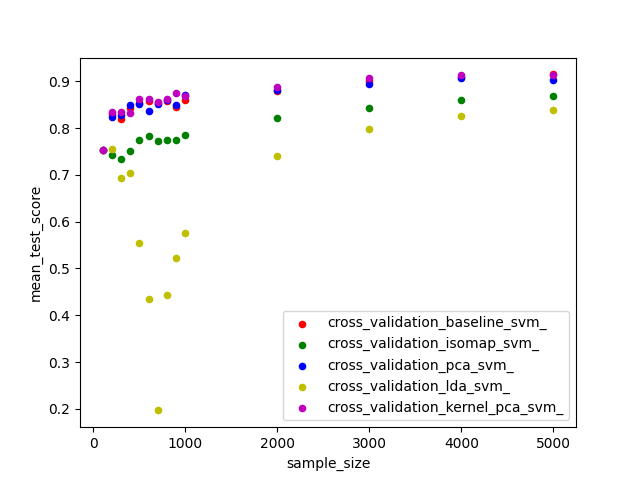
\includegraphics[width=0.8\textwidth]{figures/test_score_based_on_size.png}
    \caption{}
    \label{fig:experiment_4_performance_size}
\end{figure}


\begin{figure}[htb!]
    \centering
    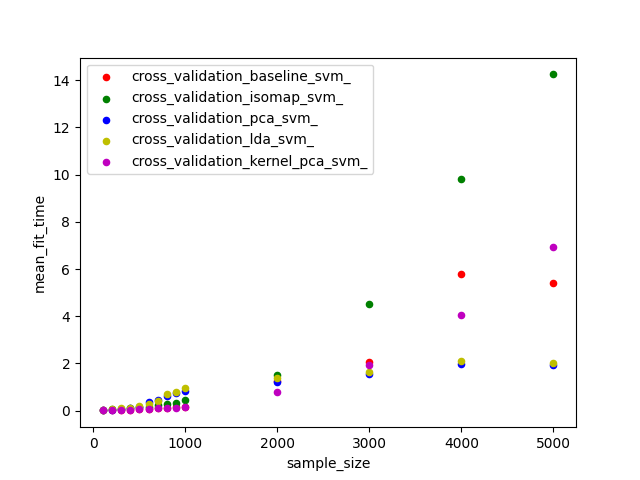
\includegraphics[width=0.8\textwidth]{figures/time_based_on_size.png}
    \caption{}
    \label{fig:experiment_4_speed_size}
\end{figure}


In terms of performance, \autoref{fig:experiment_4_performance_size} shows that both baseline \gls{pca} and \gls{kpca} perform similarly well across all sample sizes, with consistently high F1 scores. In contrast, \gls{lda} performs worse overall, while \gls{isomap} has slightly lower F1 scores in smaller sample sizes but performs better in larger samples.

In terms of speed, \autoref{fig:experiment_4_speed_size} shows that both \gls{pca} and \gls{lda} are the fastest when the sample size is larger than 2000, although they are slightly slower in smaller samples. Baseline \gls{pca} is the third slowest, while \gls{kpca} is the second slowest at a sample size of 5000. \gls{isomap} is the slowest overall, with longer runtimes for sample sizes of 2000 and above.

Overall, it appears that both \gls{pca} and \gls{kpca} are good choices for improving the performance of a \gls{svm} model on the \gls{mnist} dataset, as they offer both high performance and fast runtime. \gls{lda} may be a less optimal choice due to its lower performance, while \gls{isomap} may be a bad option for larger sample sizes but may be suitable for smaller samples due to its slower runtime.
